\documentclass[12pt]{report}
\usepackage[utf8]{inputenc}
\usepackage[margin=1.2in]{geometry}
\usepackage{graphicx}
\usepackage{float}
\usepackage{subcaption}
\usepackage{amsmath}
\usepackage{amssymb}
\usepackage{ulem}
\usepackage{bm}
\usepackage{framed}
\usepackage{xcolor}
\usepackage{ragged2e}
\usepackage{color}
\usepackage{soul}
\usepackage{cancel}
\graphicspath{ {images/} }
\setlength{\parskip}{1em}
\allowdisplaybreaks

\usepackage{titling}
\newcommand{\subtitle}[1]{%
	\posttitle{%
		\par\end{center}
	\begin{center}\large#1\end{center}
	\vskip0.5em}%
}

\newenvironment{blueframed}[1][blue]
{\def\FrameCommand{\fboxsep=\FrameSep\fcolorbox{#1}{white}}%
	\MakeFramed {\advance\hsize-\width \FrameRestore}}
{\endMakeFramed}

\newenvironment{spmatrix}[1]
{\def\mysubscript{#1}\mathop\bgroup\begin{bmatrix}}
	{\end{bmatrix}\egroup_{\textstyle\mathstrut\mysubscript}}

\title{Tutorial 7}
\subtitle
{
	\textbf{keywords}: level log interpretation, dummy variables, hypothesis test, F-test, t-test, p-value, overall significance, individual significance, multiple linear restrictions, reparameterisation
	
	\textbf{estimated reading time}: 35 minutes
}
\author{Quang Bui}
\date{Septermber 4, 2018}

\begin{document}
	
\maketitle

\section*{Question 1}
\noindent EViews workfile: \textit{vote1.wf1}

\noindent \textcolor{red}{\textit{vote1.wf1} contains data on election outcomes and campaign expenditures for 173 two-party competitive races (Democrats and Republicans) for the House of Representatives in 1988. Information about each two-party competitive race is held in the following variables:
\begin{align*}
	votea &- \%\ vote\ received\ by\ Candidate\ A \\
	expenda &- Candidate\ A’s\ campaign\ expenditure\ (\$'000) \\
	expendb &- Candidate\ B’s\ campaign\ expenditure\ (\$'000) \\
	democa &- 1\ if\ Candidate\ A\ was\ a\ democrat,\ 0\ otherwise\ (dummy\ variable)
\end{align*}
\noindent Candidate A is chosen to be the candidate whose last name is alphabetically highest.}
%%%%%%%%%% TABLE OBJECT %%%%%%%%%%
\begin{table}[H]
	\centering
	\begin{tabular}{lrrr}
		\multicolumn{1}{r}{VOTEA}&\multicolumn{1}{r}{EXPENDA}&\multicolumn{1}{r}{EXPENDB}&\multicolumn{1}{r}{DEMOCA}\\
		\multicolumn{1}{r}{$68$}&\multicolumn{1}{r}{$328.296$}&\multicolumn{1}{r}{$8.737$}&\multicolumn{1}{r}{$1$}\\
		\multicolumn{1}{r}{$62$}&\multicolumn{1}{r}{$626.377$}&\multicolumn{1}{r}{$402.477$}&\multicolumn{1}{r}{$0$}\\
		\multicolumn{1}{r}{$73$}&\multicolumn{1}{r}{$99.607$}&\multicolumn{1}{r}{$3.065$}&\multicolumn{1}{r}{$1$}\\
		\multicolumn{1}{r}{$69$}&\multicolumn{1}{r}{$319.69$}&\multicolumn{1}{r}{$26.281$}&\multicolumn{1}{r}{$0$}\\
		\multicolumn{1}{r}{$75$}&\multicolumn{1}{r}{$159.221$}&\multicolumn{1}{r}{$60.054$}&\multicolumn{1}{r}{$0$}\\
		\multicolumn{1}{r}{$69$}&\multicolumn{1}{r}{$570.155$}&\multicolumn{1}{r}{$21.393$}&\multicolumn{1}{r}{$1$}\\
		\multicolumn{1}{r}{$59$}&\multicolumn{1}{r}{$696.748$}&\multicolumn{1}{r}{$193.915$}&\multicolumn{1}{r}{$0$}\\
		\multicolumn{1}{r}{$71$}&\multicolumn{1}{r}{$638.688$}&\multicolumn{1}{r}{$7.695$}&\multicolumn{1}{r}{$1$}\\
		\multicolumn{1}{r}{$76$}&\multicolumn{1}{r}{$616.936$}&\multicolumn{1}{r}{$19.245$}&\multicolumn{1}{r}{$1$}\\
		\multicolumn{1}{r}{$73$}&\multicolumn{1}{r}{$351.687$}&\multicolumn{1}{r}{$50.532$}&\multicolumn{1}{r}{$1$}\\
		\multicolumn{1}{r}{$68$}&\multicolumn{1}{r}{$269.887$}&\multicolumn{1}{r}{$14.71$}&\multicolumn{1}{r}{$1$}\\
		\multicolumn{1}{r}{$71$}&\multicolumn{1}{r}{$269.51$}&\multicolumn{1}{r}{$95.575$}&\multicolumn{1}{r}{$1$}\\
		\multicolumn{1}{r}{$52$}&\multicolumn{1}{r}{$1440.639$}&\multicolumn{1}{r}{$1089.57$}&\multicolumn{1}{r}{$0$}\\
		\multicolumn{1}{r}{$79$}&\multicolumn{1}{r}{$252.336$}&\multicolumn{1}{r}{$69.563$}&\multicolumn{1}{r}{$1$}\\
		\multicolumn{1}{r}{$50$}&\multicolumn{1}{r}{$1470.674$}&\multicolumn{1}{r}{$1548.193$}&\multicolumn{1}{r}{$0$}\\
		\multicolumn{1}{r}{$64$}&\multicolumn{1}{r}{$140.486$}&\multicolumn{1}{r}{$100.956$}&\multicolumn{1}{r}{$1$}\\
		\multicolumn{1}{r}{$72$}&\multicolumn{1}{r}{$191.334$}&\multicolumn{1}{r}{$15.449$}&\multicolumn{1}{r}{$1$}\\
		\multicolumn{1}{r}{$68$}&\multicolumn{1}{r}{$398.597$}&\multicolumn{1}{r}{$15.239$}&\multicolumn{1}{r}{$1$}\\
		\multicolumn{1}{r}{$60$}&\multicolumn{1}{r}{$460.622$}&\multicolumn{1}{r}{$382.111$}&\multicolumn{1}{r}{$1$}\\
		\multicolumn{1}{r}{$67$}&\multicolumn{1}{r}{$457.41$}&\multicolumn{1}{r}{$20.608$}&\multicolumn{1}{r}{$1$}\\
	\end{tabular}
	\caption{Sample of the first 20 two-party competitive race.}
	%\label{tab:}
\end{table}


\newpage
\noindent \textcolor{red}
{
	Run a regression of $votea$ on a constant, $log(expenda)$, $log(expendb)$ and $democa$
}
$$votea = \beta_0 + \beta_1log(expenda) + \beta_2log(expendb) + \beta_3democa + u $$
\noindent To estimate this model from the Command window,
$$ls\ votea\ c\ log(expenda)\ log(expendb)\ democa$$
\begin{figure}[H]
	\centering
	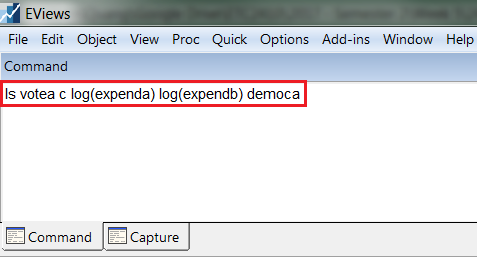
\includegraphics{q1_1}
\end{figure}
\vspace{-\baselineskip}
$$(Press\ Enter\ to\ execute\ code)$$

\noindent To name (save) the estimated equation,
$$Name \to Name\ to\ identify\ object: eq01$$
$$(This\ names\ the\ equation\ \textit{\textbf{eq01}})$$
\begin{figure}[H]
	\centering
	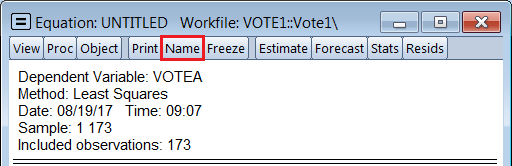
\includegraphics{q1_2}
\end{figure}
\vspace{-\baselineskip}
\begin{figure}[H]
	\centering
	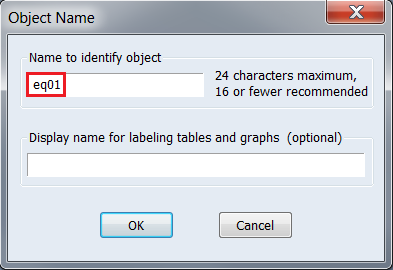
\includegraphics{q1_3}
\end{figure}
\vspace{-\baselineskip}
%%%%%%%%%% TABLE OBJECT %%%%%%%%%%
\begin{table}[H]
	\centering
	\begin{tabular}{lrrrr}
		\multicolumn{3}{l}{Dependent Variable: VOTEA}&\multicolumn{1}{c}{}&\multicolumn{1}{c}{}\\
		\multicolumn{3}{l}{Method: Least Squares}&\multicolumn{1}{c}{}&\multicolumn{1}{c}{}\\
		\multicolumn{2}{l}{Sample: 1 173}&\multicolumn{1}{c}{}&\multicolumn{1}{c}{}&\multicolumn{1}{c}{}\\
		\multicolumn{3}{l}{Included observations: 173}&\multicolumn{1}{c}{}&\multicolumn{1}{c}{}\\
		[4.5pt] \hline \\ [-4.5pt]
		\multicolumn{1}{c}{Variable}&\multicolumn{1}{r}{Coefficient}&\multicolumn{1}{r}{Std. Error}&\multicolumn{1}{r}{t-Statistic}&\multicolumn{1}{r}{Prob.}\\
		[4.5pt] \hline \\ [-4.5pt]
		\multicolumn{1}{c}{C}&\multicolumn{1}{r}{$51.13410$}&\multicolumn{1}{r}{$2.903327$}&\multicolumn{1}{r}{$17.61224$}&\multicolumn{1}{r}{$0.0000$}\\
		\multicolumn{1}{c}{LOG(EXPENDA)}&\multicolumn{1}{r}{$6.299279$}&\multicolumn{1}{r}{$0.375274$}&\multicolumn{1}{r}{$16.78582$}&\multicolumn{1}{r}{$0.0000$}\\
		\multicolumn{1}{c}{LOG(EXPENDB)}&\multicolumn{1}{r}{$-6.666045$}&\multicolumn{1}{r}{$0.391187$}&\multicolumn{1}{r}{$-17.04054$}&\multicolumn{1}{r}{$0.0000$}\\
		\multicolumn{1}{c}{DEMOCA}&\multicolumn{1}{r}{$1.208824$}&\multicolumn{1}{r}{$1.241612$}&\multicolumn{1}{r}{$0.973593$}&\multicolumn{1}{r}{$0.3317$}\\
		[4.5pt] \hline \\ [-4.5pt]
		\multicolumn{1}{l}{R-squared}&\multicolumn{1}{r}{$0.786385$}&\multicolumn{2}{l}{Mean dependent var}&\multicolumn{1}{r}{$50.50289$}\\
		\multicolumn{1}{l}{Adjusted R-squared}&\multicolumn{1}{r}{$0.782593$}&\multicolumn{2}{l}{S.D. dependent var}&\multicolumn{1}{r}{$16.78476$}\\
		\multicolumn{1}{l}{S.E. of regression}&\multicolumn{1}{r}{$7.826209$}&\multicolumn{2}{l}{Akaike info criterion}&\multicolumn{1}{r}{$6.975683$}\\
		\multicolumn{1}{l}{Sum squared resid}&\multicolumn{1}{r}{$10351.17$}&\multicolumn{2}{l}{Schwarz criterion}&\multicolumn{1}{r}{$7.048592$}\\
		\multicolumn{1}{l}{Log likelihood}&\multicolumn{1}{r}{$-599.3966$}&\multicolumn{2}{l}{Hannan-Quinn criter.}&\multicolumn{1}{r}{$7.005262$}\\
		\multicolumn{1}{l}{F-statistic}&\multicolumn{1}{r}{$207.3816$}&\multicolumn{2}{l}{Durbin-Watson stat}&\multicolumn{1}{r}{$1.652138$}\\
		\multicolumn{1}{l}{Prob(F-statistic)}&\multicolumn{1}{r}{$0.000000$}&\multicolumn{1}{c}{}&\multicolumn{1}{c}{}&\multicolumn{1}{c}{}\\
		[4.5pt] \hline \\ [-4.5pt]
	\end{tabular}
	\caption{Regression output of $votea$ on a constant, $log(expenda)$, $log(expendb)$ and $democa$.}
	%\label{tab:}
\end{table} \vspace{-\baselineskip}
\centering $\widehat{votea} = \underset{(2.9033)}{51.1341} + \underset{(0.3753)}{6.2993}log(expenda) - \underset{(0.3912)}{6.6660}log(expendb) + \underset{(1.2416)}{1.2088}democa$
$$R^2 = 0.7864$$

\newpage
\justify \noindent \textcolor{red}
{
	\uline{(a) Interpreting the regression results when explanatory variables are logarithms of the original variables and also interpreting the coefficient of dummy variables.}
}

\noindent \textcolor{red}
{
	Explain what each parameter estimate shows.
}

\justify
\begin{blueframed}
	\textcolor{blue}{\textbf{Background}}
	\vspace{-\baselineskip}
	\justify
	\textcolor{blue}{\underline{Logarithms for approximating percentage change}}
	
	\noindent \textcolor{blue}
	{
		Since, $$\dfrac{dlog(x)}{dx} = \dfrac{1}{x}$$ replacing infinitesimally small change $d$ with finite change $\Delta$ gives the approximation of $\dfrac{1}{x}$, $$\dfrac{\Delta log(x)}{\Delta x} \approx \dfrac{1}{x}$$ and by multiplying $\Delta x$ on both sides, we have the approximate proportional change in $x$, $$\Delta log(x) \approx \dfrac{\Delta x}{x}$$ Multiplying 100 on both sides gives us the approximate percentage change in $x$, \begin{align*} 
			100\Delta log(x) &\approx 100\dfrac{\Delta x}{x} \\ 
			&= \%\Delta x 
		\end{align*} Since the approximation comes from replacing infinitesimally small change $d$ with finite change $\Delta$, this means that when the finite change $\Delta$ is large, the approximation will be less precise.
	}
	\justify
	\textcolor{blue}{\underline{Level-log interpretation}}
	
	\noindent \textcolor{blue}
	{
		For the following estimated model, which is level in the dependent variable and log in $x_1$, $$\hat{y} = \hat{\beta}_0 + \hat{\beta}_1log(x_1) + \hat{\beta}_2x_2$$ the change in $\hat{y}$ depends on change in $log(x_1)$ and $x_2$, $$\Delta \hat{y} = \hat{\beta}_1\Delta log(x_1) + \hat{\beta}_2\Delta x_2$$ Multiplying $\Delta log(x_1)$ with $\dfrac{100}{100}$ gives us, $$\Delta \hat{y} = \hat{\beta}_1 \dfrac{100}{100}\Delta log(x_1) + \hat{\beta}_2\Delta x_2$$
	}
\end{blueframed}

\justify
\begin{blueframed}
	\vspace{-\baselineskip}
	\justify
	\noindent \textcolor{blue}
	{
		\begin{align*}
			\Delta \hat{y} &= \hat{\beta}_1\dfrac{100}{100}\Delta log(x_1) + \hat{\beta}_2\Delta x_2 \\
			&= \dfrac{\hat{\beta}_1}{100} 100\Delta log(x_1) + \hat{\beta}_2\Delta x_2 \\
			&= \dfrac{\hat{\beta}_1}{100} \%\Delta x_1 + \hat{\beta}_2\Delta x_2
		\end{align*}
		$\therefore$ the model estimates that if $x_2$ is held constant and $x_1$ increases by 1\%, $$\Delta x_2 = 0$$ $$\% \Delta x_1 = 1$$ on average, $y$ is estimated to change by $\dfrac{\hat{\beta}_1}{100}$, \begin{align*}
			\Delta \hat{y} &= \dfrac{\hat{\beta}_1}{100} \%\Delta x_1 + \hat{\beta}_2\Delta x_2 \\
			&= \dfrac{\hat{\beta}_1}{100} \times 1 + \hat{\beta}_2 \times 0 \\
			&= \dfrac{\hat{\beta}_1}{100}
		\end{align*} (When $x_1$ increases by 1\%, holding $x_2$ constant, the model estimates that $y$ is expected to change by $\dfrac{\hat{\beta}_1}{100}$.)
	}
\end{blueframed}
\begin{figure}[H]
	\centerline{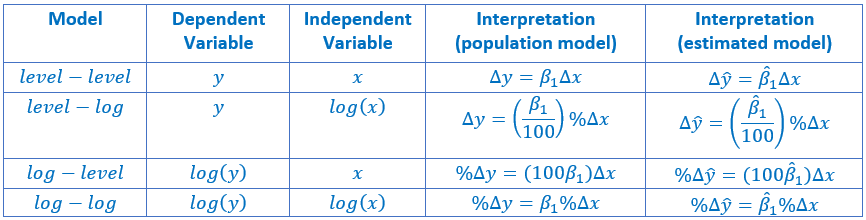
\includegraphics{tute7_q1_1}}
\end{figure}
\vspace{-\baselineskip}

\newpage
$$\widehat{votea} = \underset{(2.9033)}{51.1341} + \underset{(0.3753)}{6.2993}log(expenda) - \underset{(0.3912)}{6.6660}log(expendb) + \underset{(1.2416)}{1.2088}democa$$

\noindent $\hat{\beta}_1 = 6.2993$

\noindent The model estimates that regardless of Candidate A’s political affiliation (holding $democa$ constant) and when there is no change in Candidate B’s expenditure (holding $expendb$ constant), $$\Delta log(expendb) = 0$$ $$\Delta democa = 0$$ a 1\% increase in Candidate A’s expenditure,
$$\%{\Delta}expenda = 1\%$$ is expected to increase the share of votes received by Candidate A  by 0.063 \uline{percentage points},
\begin{align*}
	\Delta \widehat{votea} &= \hat{\beta}_1\Delta log(expenda) + \hat{\beta}_2\Delta log(expendb) + \hat{\beta}_3\Delta democa \\
	&= \hat{\beta}_1\Delta log(expenda) + \hat{\beta}_2\times 0 + \hat{\beta}_3\times 0 \\
	&= \hat{\beta}_1\Delta log(expenda) \\
	&= \dfrac{\hat{\beta}_1}{100}\%{\Delta}expenda \\
	&= \dfrac{6.2993}{100}\times1=0.063
\end{align*}


\vspace{10mm}
\noindent $\hat{\beta}_2 = -6.6660$

\noindent The model estimates that for a 1\% increase in Candidate B’s expenditure,
$$\%{\Delta}expendb = 1\%$$
the share of votes received by Candidate A is expected to decrease by 0.0667 \uline{percentage points},
$${\Delta}\widehat{votea} = \dfrac{-6.6660}{100}\times1=-0.0667$$
regardless of Candidate A’s political affiliation (holding $democa$ constant) and when there is no change in Candidate A’s expenditure (holding $expenda$ constant).


\newpage
\justify
\begin{blueframed}
	\textcolor{blue}{\textbf{Background}}
	\vspace{-\baselineskip}
	\justify
	\textcolor{blue}{\underline{Dummy variable interpretation}}
	
	\noindent \textcolor{blue} 
	{
		For the following estimated model, $$\widehat{votea} = \hat{\beta}_0 + \hat{\beta}_1log(expenda) + \hat{\beta}_2log(expendb) + \hat{\beta}_3democa$$ where $democa$ is a dummy variable, $$democa = \begin{cases}
		1 \quad if\ Candidate\ A\ was\ a\ democrat \\
		0 \quad otherwise
		\end{cases}$$ The change in $\widehat{votea}$ depends on the change in $log(expenda)$, $log(expendb)$, and $democa$, $$\Delta \widehat{votea} = \hat{\beta}_1\Delta log(expenda) + \hat{\beta}_2\Delta log(expendb) + \hat{\beta}_3\Delta democa$$ $\therefore$ the model estimates that when Candidate A and B's campaign expenditure are held constant, $$\Delta log(expenda) = 0$$ $$\Delta log(expenda) = 0$$ the share of votes received by Candidate A if Candidate A is from the Democratic party, $$\Delta democa = 1$$ is expected to be $\hat{\beta}_3$ \uline{percentage points} higher than Candidate B, \begin{align*}
		\Delta \widehat{votea} &= \hat{\beta}_1\times 0 + \hat{\beta}_2\times 0 + \hat{\beta}_3\times 1 \\
		&= \hat{\beta}_3
		\end{align*} (The model estimates that when Candidate A and B's campaign expenditure are held constant, the share of votes received by Candidate A if Candidate A is from the Democratic party is expected to be $\hat{\beta}_3$ \uline{percentage points} higher than Candidate B.)
	}
\end{blueframed}

\noindent $\hat{\beta}_3 = 1.2088$

\noindent Controlling for both candidate's campaign expenditure, the model estimates that the share of votes received by Candidate A ($votea$) if Candidate A is from the Democratic party ($democa = 1$) is expected to be 1.2088 \uline{percentage points} higher than if Candidate A were from the Republican party ($democa=0$).

\newpage
\noindent \textcolor{red}
{
	\uline{(b) Test the overall significance of a regression.}
}

\noindent \textcolor{red}
{
	Test the overall significance of the model at the 1\% significance level (ignore the fact that EViews produces the F statistic, compute it using $R^2$). Explain in words the hypothesis that you are testing.
}
$$votea = \beta_0 + \beta_1log(expenda) + \beta_2log(expendb) + \beta_3democa + u $$
\noindent A test of overall significance is a test of whether the regressors in our model jointly help explain the dependent variable. If none of the regressors jointly help to explain $votea$ then,
$$\beta_1 = \beta_2 = \beta_3 = 0$$
but if at least one of the regresors helps to explain $votea$ then,
$$at\ least\ one\ of\ \beta_1, \beta_2, \beta_3\ is\ not\ 0$$
\noindent \textbf{State the null and alternative hypothesis}
\begin{align*}
	H_0&: \beta_1 = \beta_2 = \beta_3 = 0 \\
	H_1&: at\ least\ one\ of\ \beta_1, \beta_2, \beta_3\ is\ not\ 0
\end{align*}
\noindent \textbf{The test statistic and its distribution under $H_0$}
$$F = \dfrac{R^{2}/k}{(1-R^2)/(n-k-1)} = \dfrac{R^{2}/3}{(1-R^2)/(173-3-1)} \sim F_{q,n-k-1} \quad under\ H_0$$
\begin{align*}
	n &= sample\ size \\
	k &= number\ of\ regressors\ in\ the\ model  
\end{align*}
\noindent Note: For a test of overall joint significance of a regression, the F test statistic which is usually expressed as, $$F = \dfrac{(SSR_r - SSR_{ur})/q}{SSR_{ur}/(n-k-1)}$$ can also be expressed as,
$$F = \dfrac{(SSR_r - SSR_{ur})/q}{SSR_{ur}/(n-k-1)} = \dfrac{R^{2}/k}{(1-R^2)/(n-k-1)}$$
\noindent \textbf{Calculate the test statistic}
$$F_{calc} = \dfrac{0.786385/3}{(1-0.786385)/(173-3-1)} = 207.38 $$
\begin{figure}[H]
	\centering
	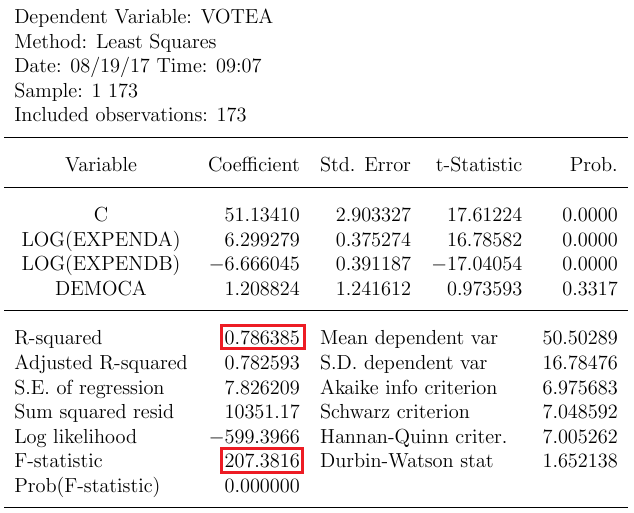
\includegraphics{q1_4}
\end{figure}
\vspace{-\baselineskip}
\noindent \textbf{Critical value and rejection region}

\noindent $1\%\ significance\ level\ \to \alpha = 0.01$

\noindent To obtain the critical value using the Stats Table, locate the F distribution table at the 1\% significance level,
$$Numerator\ d.o.f = 3$$
$$Denominator\ d.o.f = 169$$
\noindent Since 169 is not in the table, we take a conservative approach and choose the closest available degrees of freedom less than 169 i.e. $d.o.f=120$. 
\begin{figure}[H]
	\centering
	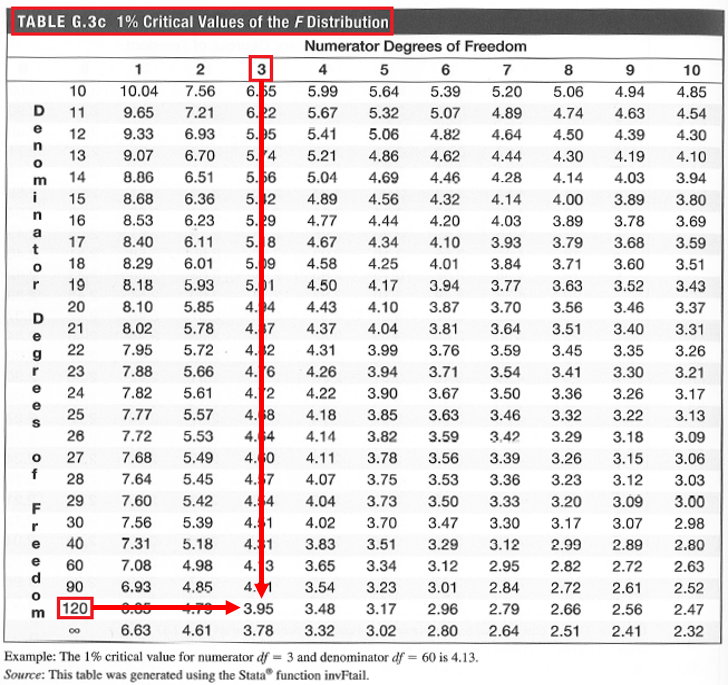
\includegraphics{q1_5}
\end{figure}
\vspace{-\baselineskip}
\noindent To obtain the critical value using EViews,
$$Command\ window:\ scalar\ cvf3\_169\_1=@qfdist(0.99,3,169)$$
\begin{figure}[H]
	\centering
	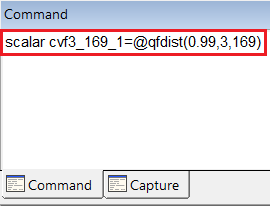
\includegraphics{q1_6}
\end{figure}
\vspace{-\baselineskip}
\begin{figure}[H]
	\centering
	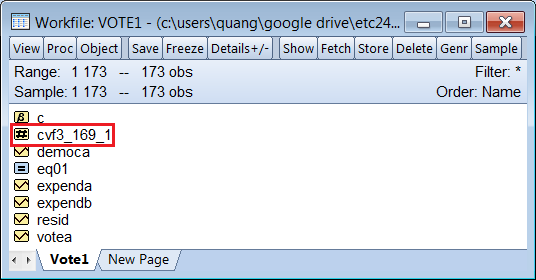
\includegraphics{q1_7}
\end{figure}
\vspace{-\baselineskip}
\begin{figure}[H]
	\centering
	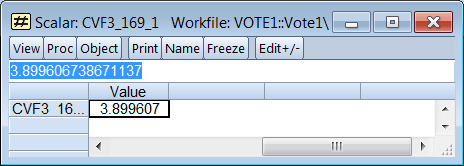
\includegraphics{q1_8}
\end{figure}
\vspace{-\baselineskip}
$$F_{crit}\ (from\ Stat\ Table) = 3.95$$
$$F_{crit}\ (from\ EViews) = 3.8996$$

\noindent We reject $H_0$ if,
$$F_{calc} > F_{crit}$$
\noindent \textbf{Conclusion}

\noindent Since $F_{calc}=207.38>F_{crit}=3.95$, we reject the null at the 1\% significance level and conclude that at least one of the regressors in the model is statistically significant in explaining the share of votes received by Candidate A.

\newpage
\noindent \textcolor{red}
{
	\uline{(c) Test of significance of an explanatory variable.}
}

\noindent \textcolor{red}
{
	Test the hypothesis that controlling for campaign expenditure, being a democratic candidate is not significant in predicting the \% of vote received in competitive races at the 5\% level of significance. Perform that test by two methods: 
	(i) comparing the t statistic with an appropriate critical value, and 
	(ii) using the p-value.
}

\noindent If after controlling for campaign expenditure, being a democratic candidate is not significant in predicting the \% of vote received then,
$$votea = \beta_0 + \beta_1log(expenda) + \beta_2log(expendb) + \xcancel{\beta_3democa} + u $$
\noindent that is,
$$\beta_3 = 0$$
\noindent but if it does then,
$$\beta_3 \neq 0$$
\noindent \textbf{State the null and alternative hypothesis}
\begin{align*}
H_0&: \beta_3 = 0 \\
H_1&: \beta_3 \neq 0
\end{align*}
\noindent \textbf{The test statistic and its distribution under $H_0$}
$$t = \dfrac{\hat{\beta}_3 - \beta_3}{se(\hat{\beta}_3)} = \dfrac{\hat{\beta}_3}{se(\hat{\beta}_3)} \sim t_{n-k-1} \quad under\ H_0$$
\begin{align*}
n &= sample\ size = 173 \\
k &= number\ of\ regressors\ in\ the\ model = 3
\end{align*}

\noindent \textbf{Calculate the test statistic}
$$t_{calc} = \dfrac{1.208824}{1.241612} = 0.9736$$
\begin{figure}[H]
	\centering
	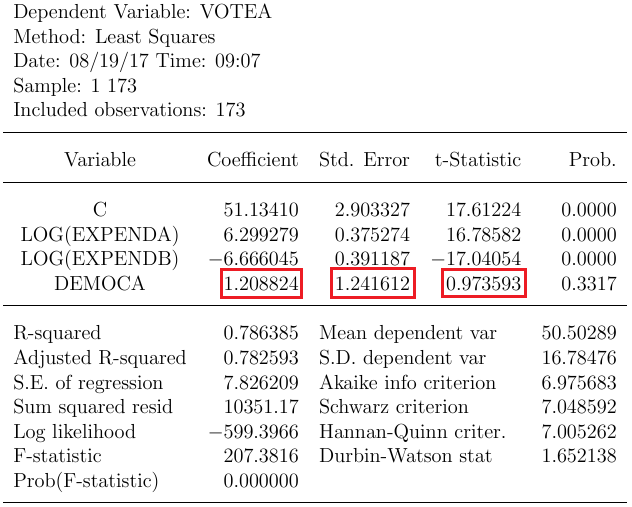
\includegraphics{q1_9}
\end{figure}
\vspace{-\baselineskip}
\noindent Note: The $t-Statistics$ from the EViews regression output are $t_{calc}$ values for a two-sided t-test to test if a regressor has a statistically significant on the dependent variable, holding the other regressors constant.

\newpage
\noindent \textbf{p-value from regression output}
\begin{figure}[H]
	\centering
	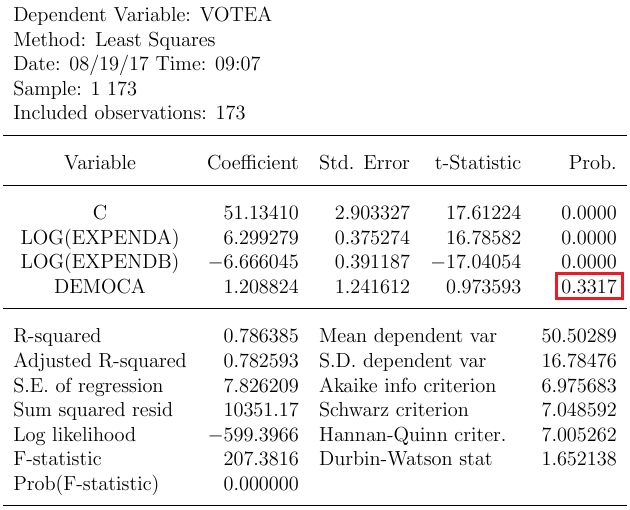
\includegraphics{q1_10}
\end{figure}
\vspace{-\baselineskip}
$$p-value = 0.3317$$
\noindent Note: The $Prob.$ values from the EViews regression output are p-values for a two-sided t-test to test if a regressor is statistically significant, holding the other regressors constant.

\noindent \textbf{Critical value and rejection region}

\noindent $5\%\ significance\ level\ \to \alpha = 0.05$

\noindent To obtain the critical value using the Stats Table, locate the t distribution table,
$$degrees\ of\ freedom = 169$$
\noindent Since 169 is not in the table, we take a conservative approach and choose the closest available degrees of freedom less than 169 i.e. $d.o.f=120$. 
\begin{figure}[H]
	\centering
	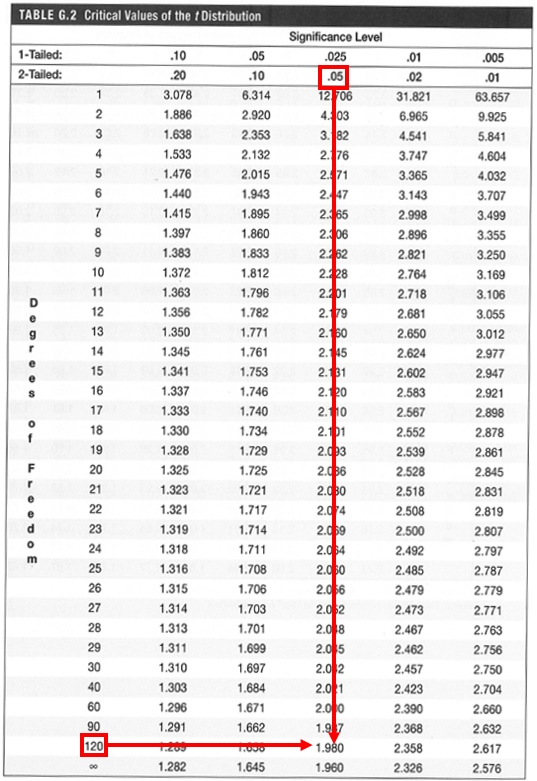
\includegraphics{q1_11}
\end{figure}
\vspace{-\baselineskip}
\noindent To obtain the critical value using EViews,
$$Command\ window:\ scalar\ cvt169\_5\_twotail=@qtdist(0.975,169)$$
\begin{figure}[H]
	\centering
	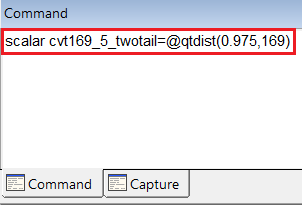
\includegraphics{q1_12}
\end{figure}
\vspace{-\baselineskip}
\begin{figure}[H]
	\centering
	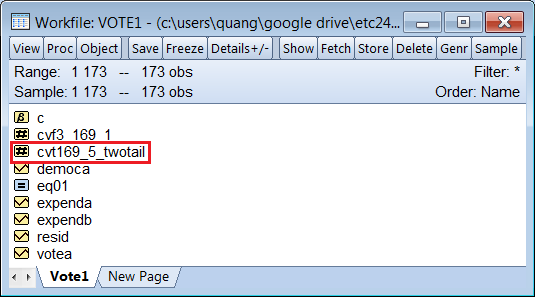
\includegraphics{q1_13}
\end{figure}
\vspace{-\baselineskip}
\begin{figure}[H]
	\centering
	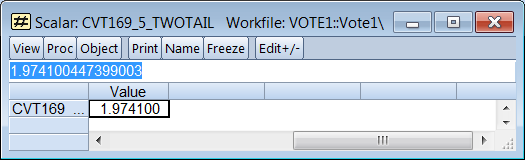
\includegraphics{q1_14}
\end{figure}
\vspace{-\baselineskip}
\noindent From Stat Table:
\begin{align*}
	+t_{crit} &= 1.980 \\
	-t_{crit} &= -1.980
\end{align*}
\noindent From EViews:
\begin{align*}
	+t_{crit} &= 1.9751 \\
	-t_{crit} &= -1.9751
\end{align*}

\noindent Rejection rule: 

\noindent Comparing the calculated test statistic with the critical value, we reject $H_0$ if,
$$t_{calc} > +t_{crit}$$
$$or$$
$$t_{calc} < -t_{crit}$$

\noindent Comparing the p-value with the significance level, we reject $H_0$ if,
$$p-value < \alpha = 0.05$$
\noindent \textbf{Conclusion}

\noindent Since $p-value = 0.3317 > \alpha = 0.05$, we do not reject the null at the 5\% significance level and conclude that there is insufficient evidence from our sample to suggest that Candidate A’s political affiliation is statistically significant in explaining the share of votes received by Candidate A, holding campaign expenditure constant.

\newpage
\noindent \textcolor{red}
{
	\uline{(d) Joint test of multiple linear restrictions.}
}

\noindent \textcolor{red}
{
	Test the joint hypothesis that controlling for campaign expenditure, being a democratic candidate does not contribute to the \% vote received and that the effect (on $votea$) of every percentage increase in campaign expenditure by Candidate A can be offset exactly by the same percentage increase in the opponent’s campaign expenditure. Perform this test at the 5\% level of significance.
}

\noindent From the statement,

\centering
“..controlling for campaign expenditure, being a democratic candidate does not contribute to the \% of vote received..”
\vspace{-\baselineskip}
\justify
we have our first linear restriction,
$$\beta_3 = 0$$

\noindent From the statement,

\centering
“..the effect (on $votea$) of every percentage increase in campaign expenditure by Candidate A can be offset exactly by the same percentage increase in the opponent’s campaign expenditure..”
\vspace{-\baselineskip}
\justify
we have our second linear restriction,
$$\beta_1 + \beta_2 = 0$$
$$\beta_2 = -\beta_1$$
\noindent It tells us that the effect on $votea$ when both Candidate's campaign expenditure increases by the same percentage equals to 0.
\vspace{10mm}

\noindent \textbf{Unrestricted model (the model before imposing restrictions)}:
$$votea = \beta_0 + \beta_1log(expenda) + \beta_2log(expendb) + \beta_3democa + u$$

\noindent \textbf{Restricted model (the model after imposing restrictions)}:
\begin{align*}
	votea &= \beta_0 + \beta_1log(expenda) - \beta_1log(expendb) + 0{\times}democa + u \\
	votea &= \beta_0 + \beta_1(log(expenda) - log(expendb)) + u
\end{align*}

\newpage
\noindent \textbf{State the null and alternative hypothesis}
\begin{align*}
	H_0&: \beta_3 = 0, \beta_2 = -\beta_1 \\
	H_1&: \beta_3 \neq 0\ and/or\ \beta_2 \neq -\beta_1
\end{align*}

\noindent \textbf{The test statistic and its distribution under $H_0$}
$$F = \dfrac{(SSR_r - SSR_{ur})/q}{SSR_{ur}/(n-k-1)} = \dfrac{(SSR_r - SSR_{ur})/2}{SSR_{ur}/(173-3-1)} \sim F_{q,n-k-1} \quad under\ H_0$$
\begin{align*}
n &= sample\ size = 173 \\
k &= number\ of\ regressors\ in\ the\ unrestricted\ model = 3 \\
q &= number\ of\ restrictions\ = 2 \\
SSR_{r} &= sum\ of\ squared\ residuals\ from\ estimated\ restricted\ model \\
SSR_{ur} &= sum\ of\ squared\ residuals\ from\ estimated\ unrestricted\ model
\end{align*}

\noindent \textbf{Calculate the test statistic}

\noindent From the regression output of the estimated unrestricted model,
$$SSR_{ur} = 10351.17$$
\begin{figure}[H]
	\centering
	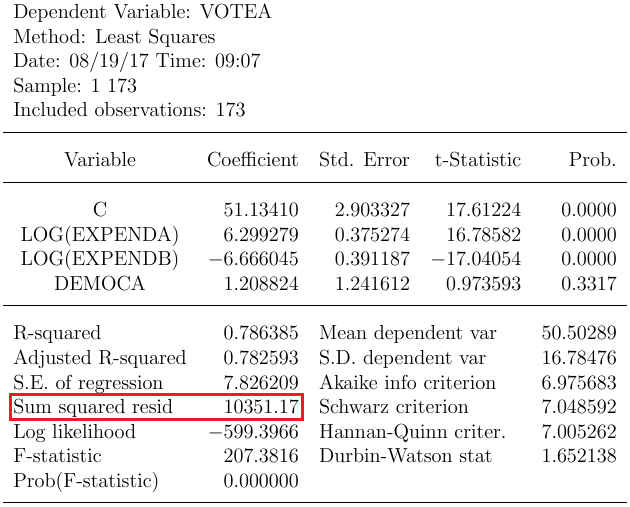
\includegraphics{q1_15}
\end{figure}
\vspace{-\baselineskip}
\noindent To obtain $SSR_r$, we need to estimate the restricted model,
$$votea = \beta_0 + \beta_1(log(expenda) - log(expendb)) + u $$
\noindent To estimate this model from the Command window,
$$ls\ votea\ c\ (log(expenda)-log(expendb))$$
\begin{figure}[H]
	\centering
	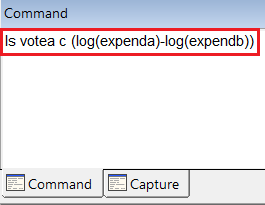
\includegraphics{q1_16}
\end{figure}
\vspace{-\baselineskip}
$$(Press\ Enter\ to\ execute\ code)$$

\noindent To name (save) the estimated equation,
$$Name \to Name\ to\ identify\ object: eq02$$
$$(This\ names\ the\ equation\ \textit{\textbf{eq02}})$$
\begin{figure}[H]
	\centering
	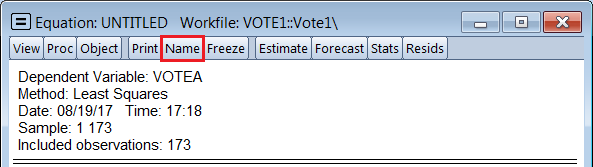
\includegraphics{q1_17}
\end{figure}
\vspace{-\baselineskip}
\begin{figure}[H]
	\centering
	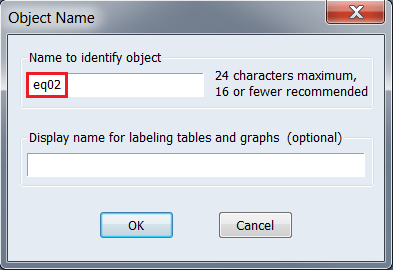
\includegraphics{q1_18}
\end{figure}
\vspace{-\baselineskip}
%%%%%%%%%% TABLE OBJECT %%%%%%%%%%
\begin{table}[H]
	\centering
	\begin{tabular}{lrrrr}
		\multicolumn{3}{l}{Dependent Variable: VOTEA}&\multicolumn{1}{c}{}&\multicolumn{1}{c}{}\\
		\multicolumn{3}{l}{Method: Least Squares}&\multicolumn{1}{c}{}&\multicolumn{1}{c}{}\\
		\multicolumn{3}{l}{Date: 08/19/17   Time: 17:18}&\multicolumn{1}{c}{}&\multicolumn{1}{c}{}\\
		\multicolumn{2}{l}{Sample: 1 173}&\multicolumn{1}{c}{}&\multicolumn{1}{c}{}&\multicolumn{1}{c}{}\\
		\multicolumn{3}{l}{Included observations: 173}&\multicolumn{1}{c}{}&\multicolumn{1}{c}{}\\
		[4.5pt] \hline \\ [-4.5pt]
		\multicolumn{1}{c}{Variable}&\multicolumn{1}{r}{Coefficient}&\multicolumn{1}{r}{Std. Error}&\multicolumn{1}{r}{t-Statistic}&\multicolumn{1}{r}{Prob.}\\
		[4.5pt] \hline \\ [-4.5pt]
		\multicolumn{1}{c}{C}&\multicolumn{1}{r}{$49.97148$}&\multicolumn{1}{r}{$0.594598$}&\multicolumn{1}{r}{$84.04253$}&\multicolumn{1}{r}{$0.0000$}\\
		\multicolumn{1}{c}{LOG(EXPENDA)-LOG(EXPENDB)}&\multicolumn{1}{r}{$6.545465$}&\multicolumn{1}{r}{$0.262391$}&\multicolumn{1}{r}{$24.94545$}&\multicolumn{1}{r}{$0.0000$}\\
		[4.5pt] \hline \\ [-4.5pt]
		\multicolumn{1}{l}{R-squared}&\multicolumn{1}{r}{$0.784438$}&\multicolumn{2}{l}{Mean dependent var}&\multicolumn{1}{r}{$50.50289$}\\
		\multicolumn{1}{l}{Adjusted R-squared}&\multicolumn{1}{r}{$0.783178$}&\multicolumn{2}{l}{S.D. dependent var}&\multicolumn{1}{r}{$16.78476$}\\
		\multicolumn{1}{l}{S.E. of regression}&\multicolumn{1}{r}{$7.815690$}&\multicolumn{2}{l}{Akaike info criterion}&\multicolumn{1}{r}{$6.961637$}\\
		\multicolumn{1}{l}{Sum squared resid}&\multicolumn{1}{r}{$10445.54$}&\multicolumn{2}{l}{Schwarz criterion}&\multicolumn{1}{r}{$6.998091$}\\
		\multicolumn{1}{l}{Log likelihood}&\multicolumn{1}{r}{$-600.1816$}&\multicolumn{2}{l}{Hannan-Quinn criter.}&\multicolumn{1}{r}{$6.976426$}\\
		\multicolumn{1}{l}{F-statistic}&\multicolumn{1}{r}{$622.2757$}&\multicolumn{2}{l}{Durbin-Watson stat}&\multicolumn{1}{r}{$1.657779$}\\
		\multicolumn{1}{l}{Prob(F-statistic)}&\multicolumn{1}{r}{$0.000000$}&\multicolumn{1}{c}{}&\multicolumn{1}{c}{}&\multicolumn{1}{c}{}\\
		[4.5pt] \hline \\ [-4.5pt]
	\end{tabular}
	\caption{Regression output of $votea$ on a constant and $log(expenda)-log(expendb)$.}
	%\label{tab:}
\end{table}
\vspace{-\baselineskip}
\centering $SSR_r = 10445.54$
$$F_{calc} = \dfrac{(SSR_r - SSR_{ur})/2}{SSR_{ur}/(173-3-1)} = \dfrac{(10445.54-10351.17)/2}{10351.17/(169)} = 0.77 $$

\justify \noindent \textbf{Critical value and rejection region}

\noindent $5\%\ significance\ level\ \to \alpha = 0.05$

\noindent To obtain the critical value using the Stats Table, locate the F distribution table at the 5\% significance level,
$$Numerator\ d.o.f = 2$$
$$Denominator\ d.o.f = 169$$
\noindent Since 169 is not in the table, we take a conservative approach and choose the closest available degrees of freedom less than 169 i.e. $d.o.f=120$. 
\begin{figure}[H]
	\centering
	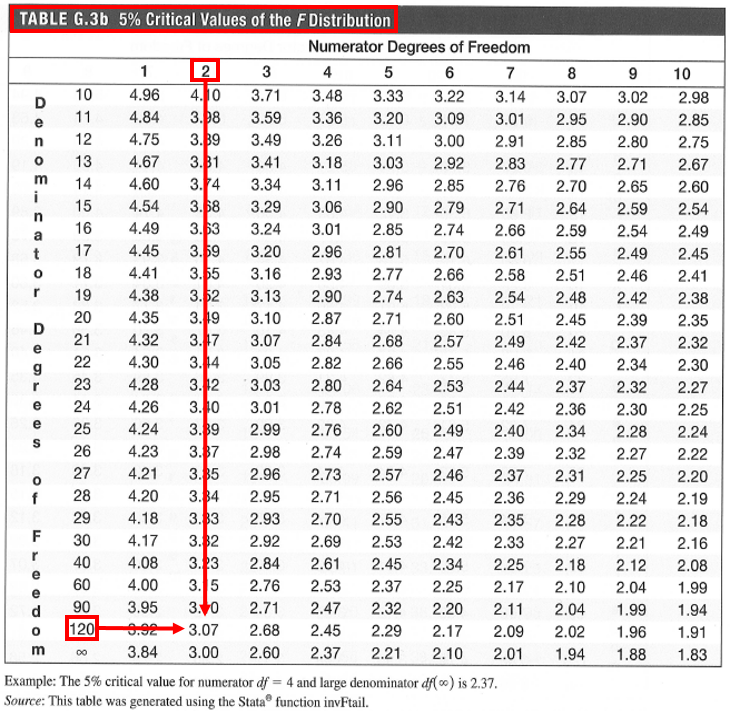
\includegraphics{q1_19}
\end{figure}
\vspace{-\baselineskip}
\noindent To obtain the critical value using EViews,
$$Command\ window:\ scalar\ cvf2\_169\_5=@qfdist(0.95,2,169)$$
\begin{figure}[H]
	\centering
	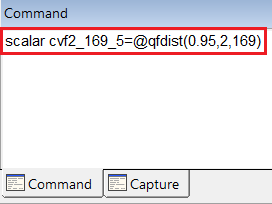
\includegraphics{q1_20}
\end{figure}
\vspace{-\baselineskip}
\begin{figure}[H]
	\centering
	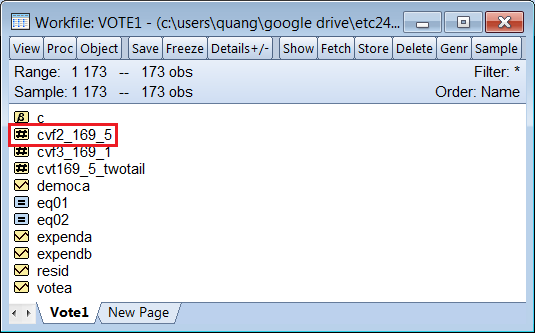
\includegraphics{q1_21}
\end{figure}
\vspace{-\baselineskip}
\begin{figure}[H]
	\centering
	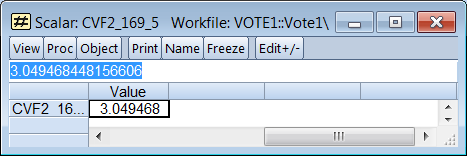
\includegraphics{q1_22}
\end{figure}
\vspace{-\baselineskip}
$$F_{crit}\ (from\ Stat\ Table) = 3.07$$
$$F_{crit}\ (from\ EViews) = 3.049$$

\noindent Rejection rule: 

\noindent Comparing the calculated test statistic with the critical value, we reject $H_0$ if,
$$F_{calc} > F_{crit}$$
\noindent \textbf{Conclusion}

\noindent Since $F_{calc}=0.77 < F_{crit}=3.95$, we do not reject the null at the 5\% significance level and conclude that there is insufficient evidence to reject the assumption that being a democratic candidate has no impact on share of votes holding campaign expenditure constant \textbf{and} that the effect on share of votes received by Candidate A from a percentage increase in Candidate A’s campaign expenditure can be offset exactly by the same percentage increase in Candidate B’s campaign expenditure.

\newpage
\noindent \textcolor{red}
{
	\uline{(e) Testing a single hypothesis about a linear combination of parameters.}
}

\noindent \textcolor{red}
{
	Drop $democa$ from the model.
}
$$votea = \beta_0 + \beta_1log(expenda) + \beta_2log(expendb) + u $$
\noindent \textcolor{red}
{
	In close races each candidate believes that he or she needs to increase their campaign expenditure by more than 1\% to offset the effect of a 1\% increase in their opponent’s expenditure. The null hypothesis is,
	$$H_0: \beta_1 + \beta_2 = 0$$ 
	and although it involves two parameters, it tests only one restriction. The alternative is, 
	$$H_1: \beta_1 + \beta_2 < 0$$ 
}

\noindent That is, the impact on the share of votes received by Candidate A for a 1\% increase in Candidate A’s campaign expenditure is not enough to offset the impact from a 1\% increase in Candidate B’s campaign expenditure on the share of votes received by Candidate A. Candidate A needs to increase their campaign expenditure by more than 1\% increase to  offset the effect of a 1\% increase in Candidate B's campaign expenditure.

\noindent \textcolor{red}
{
	so we cannot use the F test because F test provides inference against $\beta_1 + \beta_2 \neq 0$. In such cases that we have only one restriction about a linear combination, we use a reparameterisation trick: 
	$$Define\ \delta = \beta_1 + \beta_2 \implies \beta_2 = \delta - \beta_1$$
	Subsitute for $\beta_2$ in the population model and re-arrange, you will see that $\delta$ becomes the coefficient of one of the explanatory variables in the reparameterised model.
	You can see that testing $\delta = 0$ against $\delta < 0$ can be performed with a simple t test in this reparameterised model.
}

\noindent \textbf{Reparameterised model}
\begin{align*}
	votea &= \beta_0 + \beta_1log(expenda) + \beta_2log(expendb) + u \\
	&= \beta_0 + \beta_1log(expenda) + (\delta - \beta_1)log(expendb) + u \\
	&= \beta_0 + \beta_1log(expenda) + {\delta}log(expendb) - \beta_1log(expendb) + u \\
	&= \beta_0 + \beta_1(log(expenda)-log(expendb)) + {\delta}log(expendb) + u
\end{align*}

\newpage
\noindent To estimate the reparameterised model from the Command window in EViews,
$$ls\ votea\ c\ (log(expenda)-log(expendb))\ log(expendb)$$
\begin{figure}[H]
	\centering
	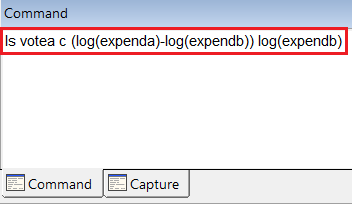
\includegraphics{q1_23}
\end{figure}
\vspace{-\baselineskip}
$$(Press\ Enter\ to\ execute\ code)$$
%%%%%%%%%% TABLE OBJECT %%%%%%%%%%
\begin{table}[H]
	\centering
	\begin{tabular}{lrrrr}
		\multicolumn{3}{l}{Dependent Variable: VOTEA}&\multicolumn{1}{c}{}&\multicolumn{1}{c}{}\\
		\multicolumn{3}{l}{Method: Least Squares}&\multicolumn{1}{c}{}&\multicolumn{1}{c}{}\\
		\multicolumn{2}{l}{Sample: 1 173}&\multicolumn{1}{c}{}&\multicolumn{1}{c}{}&\multicolumn{1}{c}{}\\
		\multicolumn{3}{l}{Included observations: 173}&\multicolumn{1}{c}{}&\multicolumn{1}{c}{}\\
		[4.5pt] \hline \\ [-4.5pt]
		\multicolumn{1}{c}{Variable}&\multicolumn{1}{r}{Coefficient}&\multicolumn{1}{r}{Std. Error}&\multicolumn{1}{r}{t-Statistic}&\multicolumn{1}{r}{Prob.}\\
		[4.5pt] \hline \\ [-4.5pt]
		\multicolumn{1}{c}{C}&\multicolumn{1}{r}{$52.03893$}&\multicolumn{1}{r}{$2.750137$}&\multicolumn{1}{r}{$18.92231$}&\multicolumn{1}{r}{$0.0000$}\\
		\multicolumn{1}{c}{LOG(EXPENDA)-LOG(EXPENDB)}&\multicolumn{1}{r}{$6.341950$}&\multicolumn{1}{r}{$0.372649$}&\multicolumn{1}{r}{$17.01858$}&\multicolumn{1}{r}{$0.0000$}\\
		\multicolumn{1}{c}{LOG(EXPENDB)}&\multicolumn{1}{r}{$-0.414801$}&\multicolumn{1}{r}{$0.538688$}&\multicolumn{1}{r}{$-0.770019$}&\multicolumn{1}{r}{$0.4424$}\\
		[4.5pt] \hline \\ [-4.5pt]
		\multicolumn{1}{l}{R-squared}&\multicolumn{1}{r}{$0.785187$}&\multicolumn{2}{l}{Mean dependent var}&\multicolumn{1}{r}{$50.50289$}\\
		\multicolumn{1}{l}{Adjusted R-squared}&\multicolumn{1}{r}{$0.782660$}&\multicolumn{2}{l}{S.D. dependent var}&\multicolumn{1}{r}{$16.78476$}\\
		\multicolumn{1}{l}{S.E. of regression}&\multicolumn{1}{r}{$7.825009$}&\multicolumn{2}{l}{Akaike info criterion}&\multicolumn{1}{r}{$6.969716$}\\
		\multicolumn{1}{l}{Sum squared resid}&\multicolumn{1}{r}{$10409.23$}&\multicolumn{2}{l}{Schwarz criterion}&\multicolumn{1}{r}{$7.024397$}\\
		\multicolumn{1}{l}{Log likelihood}&\multicolumn{1}{r}{$-599.8804$}&\multicolumn{2}{l}{Hannan-Quinn criter.}&\multicolumn{1}{r}{$6.991900$}\\
		\multicolumn{1}{l}{F-statistic}&\multicolumn{1}{r}{$310.6936$}&\multicolumn{2}{l}{Durbin-Watson stat}&\multicolumn{1}{r}{$1.662940$}\\
		\multicolumn{1}{l}{Prob(F-statistic)}&\multicolumn{1}{r}{$0.000000$}&\multicolumn{1}{c}{}&\multicolumn{1}{c}{}&\multicolumn{1}{c}{}\\
		[4.5pt] \hline \\ [-4.5pt]
	\end{tabular}
	%\caption{Regression output of $votea$ on a constant, $log(expenda)-log(expendb)$ and $log(expendb)$.}
	%\label{tab:}
\end{table} \begin{align*}
	\widehat{votea} &= \underset{(se(\hat{\beta}_0))}{\hat{\beta}_0} + \underset{(se(\hat{\beta}_1))}{\hat{\beta}_1}(log(expenda)-log(expendb)) + \underset{(se(\hat{\delta}))}{\hat{\delta}}log(expendb) \\ 
	\widehat{votea} &= \underset{(2.7501))}{52.0389} + \underset{(0.3726))}{6.3420}(log(expenda)-log(expendb)) - \underset{(0.5387)}{0.4148}log(expendb)
\end{align*}

\noindent \textbf{State the null and alternative hypothesis}
\begin{align*}
H_0&: \delta = 0 \quad (same\ as\ \beta_1 + \beta_2 = 0) \\
H_1&: \delta < 0 \quad (same\ as\ \beta_1 + \beta_2 < 0)
\end{align*}
$$(one-sided\ t\ test)$$
\noindent \textbf{The test statistic and its distribution under $H_0$}
$$t = \dfrac{\hat{\delta} - \delta}{se(\hat{\delta})} = \dfrac{\hat{\delta}}{se(\hat{\delta})} \sim t_{n-k-1} \quad under\ H_0$$
\begin{align*}
n &= sample\ size = 173 \\
k &= number\ of\ regressors\ in\ the\ model = 2
\end{align*}

\noindent \textbf{Calculate the test statistic}
$$t_{calc} = \dfrac{-0.414801}{0.538688} = -0.77$$


\noindent \textbf{p-value}
$$p-value = \dfrac{0.4424}{2} = 0.2212$$

\noindent Note: The $Prob.$ values from the EViews regression output are p-values for a two-sided t-tests of individual significance so to calculate the p-value for our one-sided t-test, we divided the two-sided p-value by 2.

\begin{figure}[H]
	\centering
	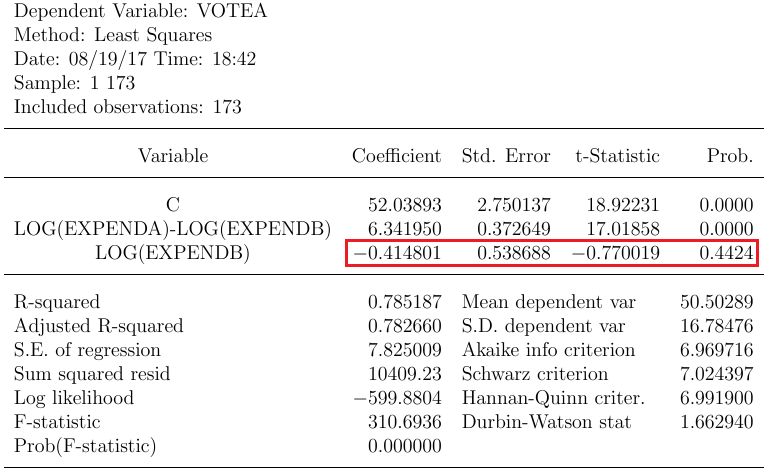
\includegraphics{q1_27}
\end{figure}
\vspace{-\baselineskip}

\noindent \textbf{Critical value and rejection region}

\noindent $5\%\ significance\ level\ \to \alpha = 0.05$

\noindent To obtain the critical value using the Stats Table, locate the t distribution table,
$$degrees\ of\ freedom = 170$$
\noindent Since 170 is not in the table, we take a conservative approach and choose the closest available degrees of freedom less than 170 i.e. $d.o.f=120$. 
\begin{figure}[H]
	\centering
	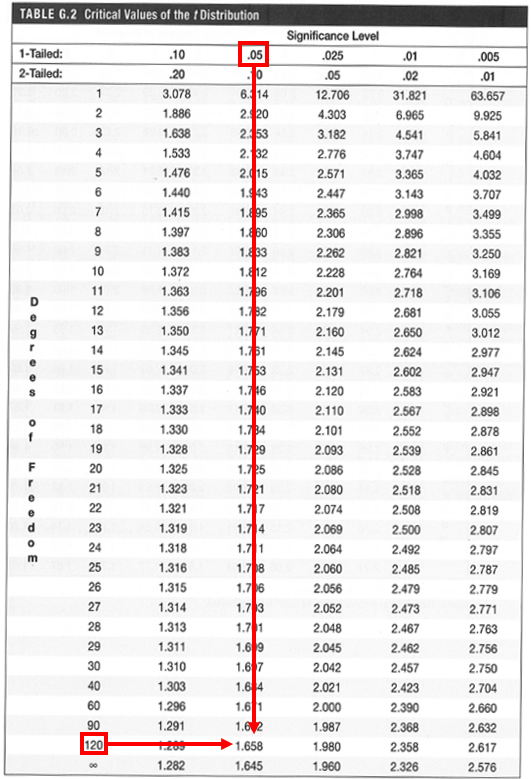
\includegraphics{q1_24}
\end{figure}
\vspace{-\baselineskip}
$$Note:This\ gives\ us\ +t_{crit}\ but\ we\ need\ -t_{crit}\ for\ this\ test$$
\noindent To obtain the critical value using EViews,
$$Command\ window:\ scalar\ cvt170\_5\_onetail=@qtdist(0.05,170)$$
\begin{figure}[H]
	\centering
	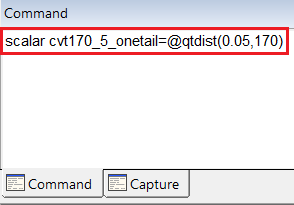
\includegraphics{q1_25}
\end{figure}
\vspace{-\baselineskip}
\begin{figure}[H]
	\centering
	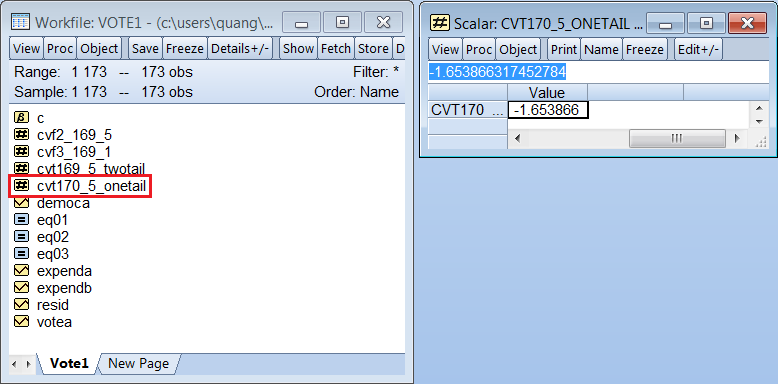
\includegraphics{q1_26}
\end{figure}
\vspace{-\baselineskip}
\noindent From Stat Table:
$$-t_{crit} = -1.658$$
\noindent From EViews:
$$-t_{crit} = -1.6539$$

\noindent Rejection rule: 

\noindent Comparing the calculated test statistic with the critical value, we reject $H_0$ if,
$$t_{calc} < -t_{crit}$$

\noindent Comparing the p-value with the significance level, we reject $H_0$ if,
$$p-value < \alpha = 0.05$$

\newpage
\noindent \textbf{Conclusion}

\noindent Since $t_{calc} =-0.77 > -t_{crit} = -1.658$, we do not reject the null at the 5\% significance level and conclude that there is insufficient evidence from our sample to suggest that Candidate A needs a larger than 1\% increase in campaign expenditure to offset the effect of a 1\% increase in Candidate B’s campaign expenditure on share of votes received by Candidate A.

\end{document}